\chapter{Conceito do projeto do portfólio}
\label{chap:fundteor}
%--------- NEW SECTION ----------------------
A concepção deste portfólio digital baseia-se em pilares fundamentais de design e comunicação digital, alinhados às necessidades específicas do cliente e às melhores práticas do mercado, com um foco particular na arquitetura e interação do sistema.

Além do mais, o projeto busca não apenas atender às expectativas do cliente, mas também proporcionar uma experiência de usuário intuitiva e eficiente, refletindo a identidade profissional do usuário.

% isso é igual <=  === <> #{ #( www
% <| |>
% ===

%conferir se precisa de requisitos do cliente
\section{Requisitos do cliente}
O cliente expressou a necessidade de um portfólio digital que atenda às seguintes especificações:
 \begin{itemize}
    \item Destaque dos serviços prestados, como refrigeração, hidráulica, elétrica, alvenaria e acabamento;
    \item Exibição de certificações e experiências relevantes;
    \item Galeria de trabalhos realizados, com imagens e descrições;
    \item Facilidade de contato, com formulários e links diretos para WhatsApp e e-mail;
    \item Seção sobre o profissional com informações pessoais e profissionais;
    \item Seção de serviços, detalhando cada área de atuação;
 \end{itemize}

 \section{Requisitos funcionais}
Os requisitos funcionais do portfólio digital incluem:
\begin{itemize}
    \item Exibição de uma página inicial com uma visão geral dos serviços;
    \item Implementação de uma galeria de imagens dos trabalhos realizados;
    \item Criação de uma seção de contato com formulários e links diretos;
    \item Inclusão de uma seção "Sobre mim" com informações pessoais e profissionais;
    \item Desenvolvimento de uma seção dedicada aos serviços, com descrições detalhadas;
    \item Implementação de um sistema de navegação intuitivo e responsivo.
\end{itemize}

%  \section{Missão}
%  \lipsum
%  %desenvolver mais
%  Além disso, o Walker deve realizar um desafio, que consiste em navegar de forma autônoma, se localizar por meio de tags e encontrar um determinado objeto.



\section{Pesquisa por similares}

A pesquisa por portfólios digitais similares não revelou tantos exemplos de profissionais autônomos na área de manutenção residencial, mas foram encontrados alguns portfólios de profissionais que atuam em áreas correlatas, como design, fotografia e serviços técnicos. Esses portfólios apresentam características comuns que podem ser adaptadas para o contexto do cliente.
A seguir, são apresentadas algumas características comuns observadas nesses portfólios:
\begin{itemize}
    \item Design responsivo e adaptável a diferentes dispositivos;
    \item Navegação intuitiva com menus claros e acessíveis;
    \item Uso de imagens de alta qualidade para destacar trabalhos realizados;
    \item Seções bem definidas para serviços, contato e informações pessoais;
    \item Integração com plataformas de comunicação.
\end{itemize}

\begin{figure}[H]
    \centering
    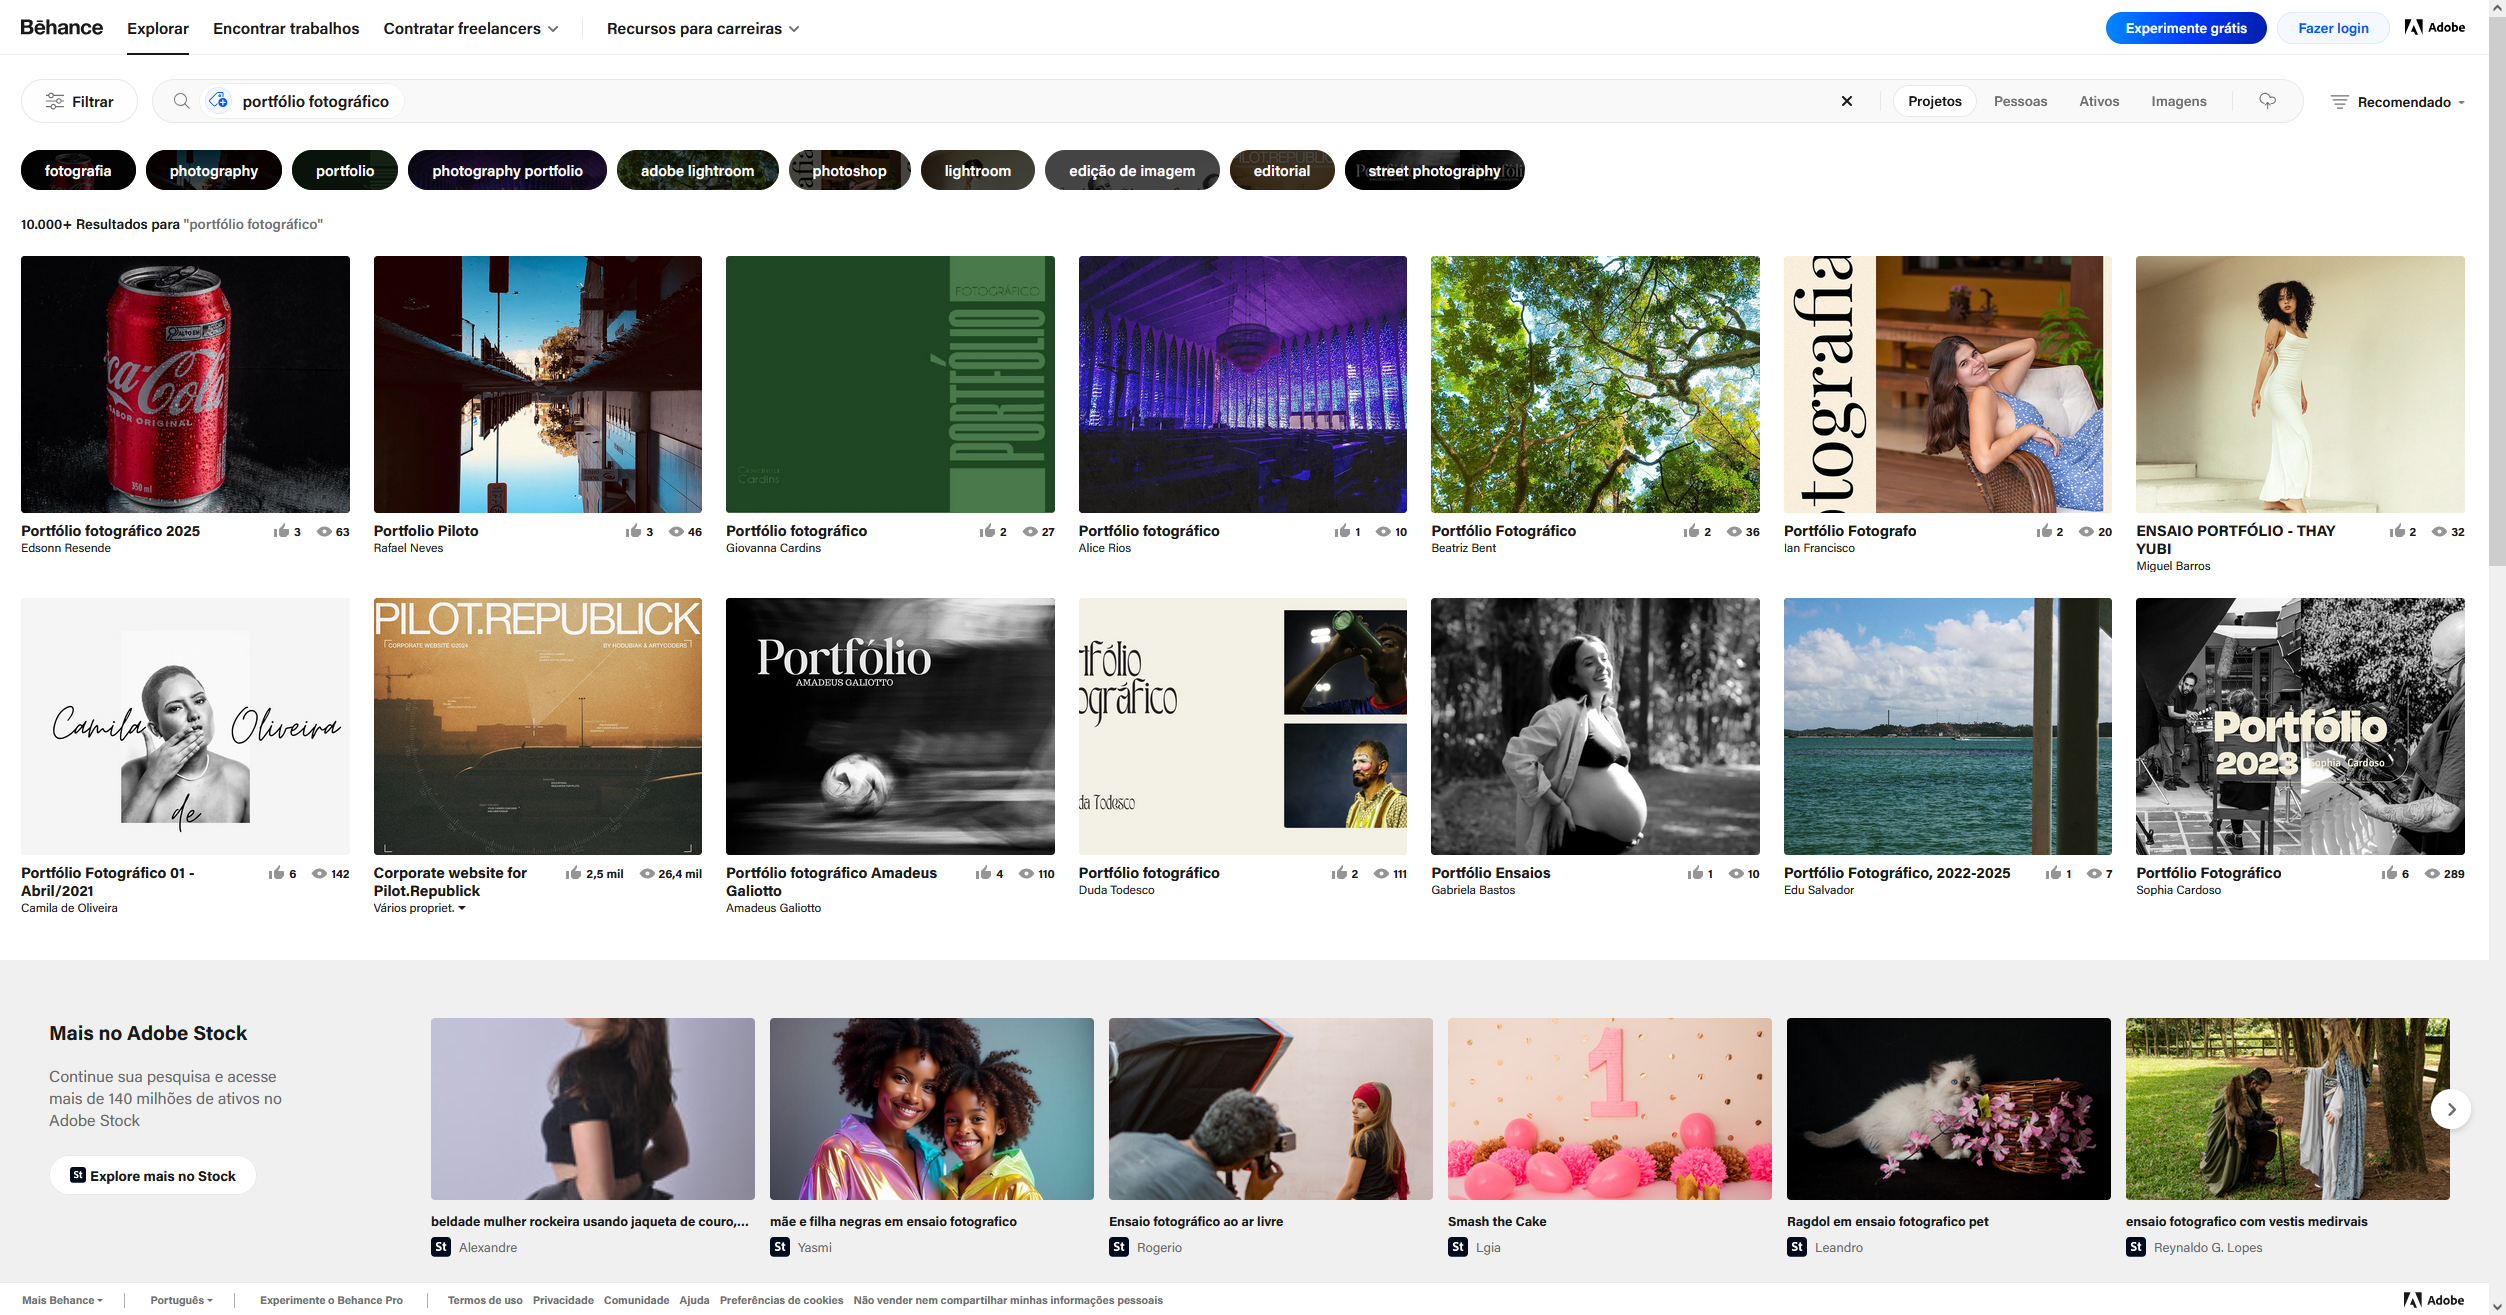
\includegraphics[width=0.6\textwidth]{Figures/foto.png} % use your image path and name here
    \caption{Exemplo de portfólio digital similar.}
    \label{fig:exemplo1-portfolio}
\end{figure}

\begin{figure}[H]
    \centering
    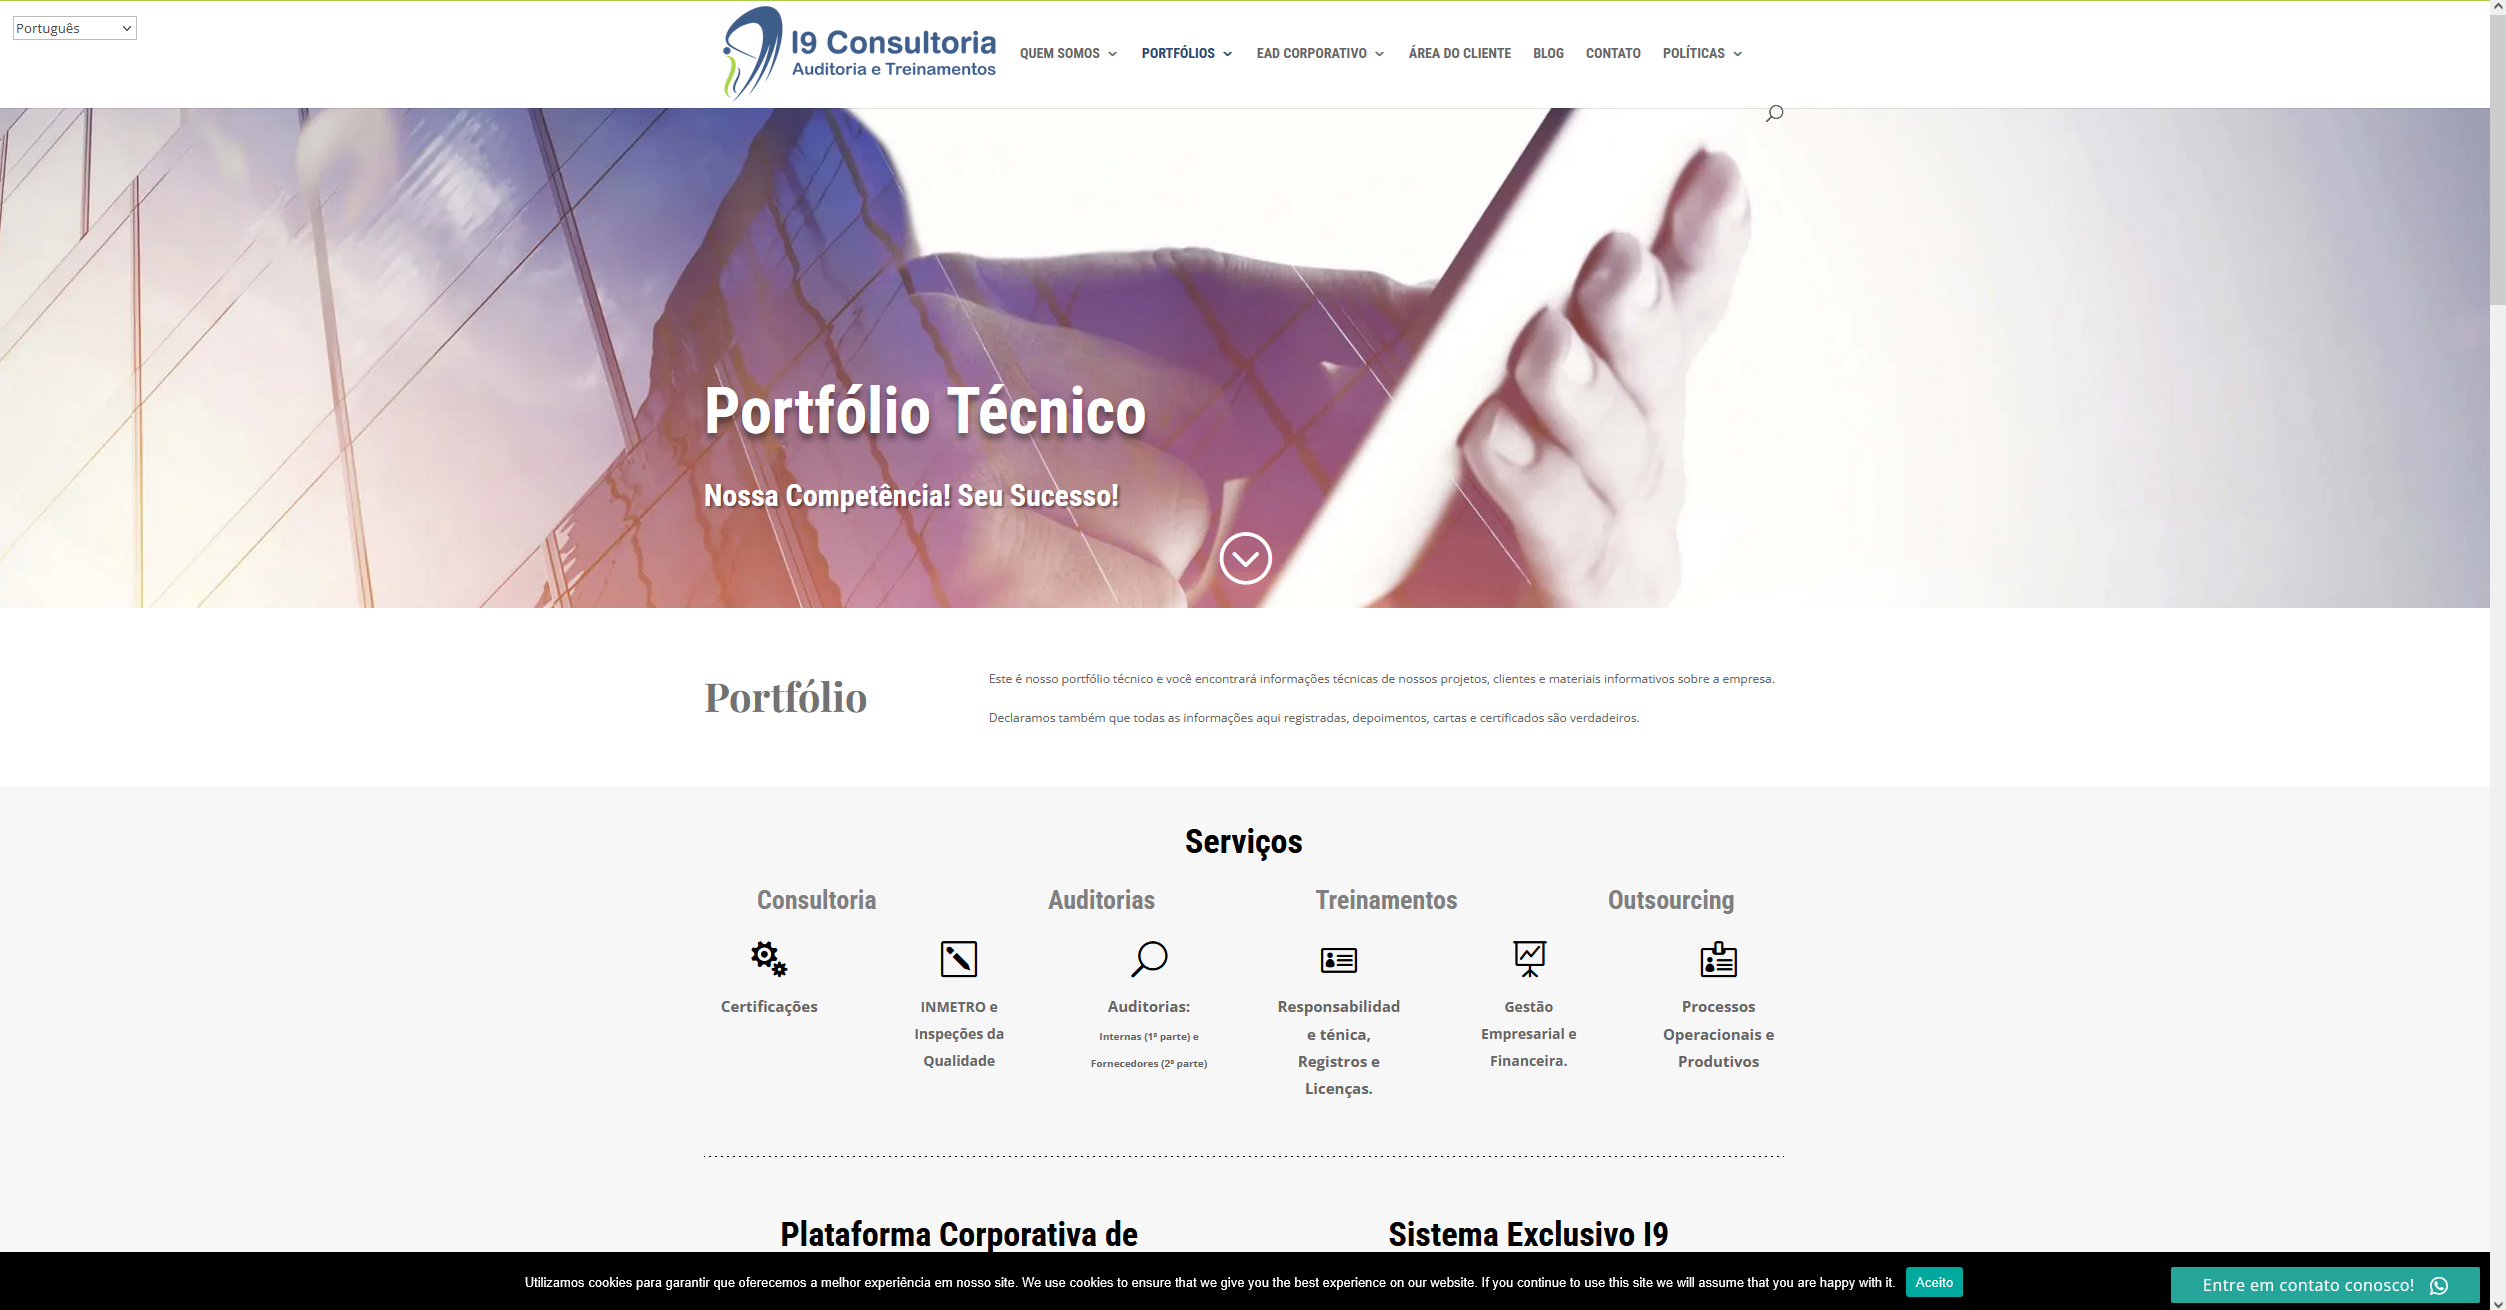
\includegraphics[width=0.6\textwidth]{Figures/trec.png} % use your image path and name here
    \caption{Exemplo de portfólio digital similar.}
    \label{fig:exemplo2-portfolio}
\end{figure}




% %----------------------------------------------------------

% %--------- NEW SECTION ----------------------


% %---------------picture------------------------------------
% % \begin{figure}
% %     \centering
% %     \subfigure[Figure A]{\label{fig:a}
\includegraphics[width=60mm]{./lq}}
% %     \subfigure[Figure B]{\label{fig:b}
\includegraphics[width=60mm]{./lq}}
% %     \subfigure[Figure C]{\label{fig:c}
\includegraphics[width=\textwidth]{./lq}}
% %     \caption{Three simple graphs}
% %     \label{fig:three graphs}
% % \end{figure}
% %----------------------------------------------------------

% % \begin{figure}
% %     \centering
% %     \begin{subfigure}[b]{0.3\textwidth}
% %         \centering
% %         
\includegraphics[width=\textwidth]{./lq}
% %         \caption{$y=x$}
% %         \label{fig:y equals x}
% %     \end{subfigure}
% %     \hfill
% %     \begin{subfigure}[b]{0.3\textwidth}
% %         \centering
% %         
\includegraphics[width=\textwidth]{./lq}
% %         \caption{$y=3sinx$}
% %         \label{fig:three sin x}
% %     \end{subfigure}
% %     \hfill
% %     \begin{subfigure}[b]{0.3\textwidth}
% %         \centering
% %         
\includegraphics[width=\textwidth]{./lq}
% %         \caption{$y=5/x$}
% %         \label{fig:five over x}
% %     \end{subfigure}
% %        \caption{Three simple graphs}
% %        \label{fig:three graphs}
% % \end{figure}


% % %--------- NEW SECTION ----------------------
% % \section{Assunto 2}
% % \label{sec:ass2}
% % flkjasdlkfjasdlkfjs

% % \begin{table}[h]
% %     \begin{subtable}[h]{0.45\textwidth}
% %         \centering
% %         \begin{tabular}{l | l | l}
% %         Day & Max Temp & Min Temp \\
% %         \hline \hline
% %         Mon & 20 & 13\\
% %         Tue & 22 & 14\\
% %         Wed & 23 & 12\\
% %         Thurs & 25 & 13\\
% %         Fri & 18 & 7\\
% %         Sat & 15 & 13\\
% %         Sun & 20 & 13
% %        \end{tabular}
% %        \caption{First Week}
% %        \label{tab:week1}
% %     \end{subtable}
% %     \hfill
% %     \begin{subtable}[h]{0.45\textwidth}
% %         \centering
% %         \begin{tabular}{l | l | l}
% %         Day & Max Temp & Min Temp \\
% %         \hline \hline
% %         Mon & 17 & 11\\
% %         Tue & 16 & 10\\
% %         Wed & 14 & 8\\
% %         Thurs & 12 & 5\\
% %         Fri & 15 & 7\\
% %         Sat & 16 & 12\\
% %         Sun & 15 & 9
% %         \end{tabular}
% %         \caption{Second Week}
% %         \label{tab:week2}
% %      \end{subtable}
% %      \caption{Max and min temps recorded in the first two weeks of July}
% %      \label{tab:temps}
% % \end{table}